
\documentclass[11pt]{article}
%Gummi|065|=)
\title{\textbf{EV 1-5 Caracteristicas de los convertidores de Potencia CA-CD, CD-CA, CA-CA y CD-CD.}} 
\author{Luis Angel Torres Pinto.\\Universidad Polit\'ecnica de la Zona Metropolitana de Guadalajara.\\Ingenier\'ia Mecatr\'onica.}
\date{16/09/2019}
\usepackage{graphicx}
\usepackage{hyperref}
\begin{document}
\maketitle
\begin{figure}[htp]
\centering

\includegraphics[scale=1.10]{UPZMG.png}
\caption{}
\label{}
\end{figure}
\section{Convertidor de Potencia CA-CD.}
Es un convertidor de corriente alterna a corriente directa basicamente parte de un rectificador de onda completa. Una de sus caracteristica es que su carga puede ser puramente resistiva. Al agregarle un capacitor en paralelo el convertidor se comporta como un filtro ya que se produce un voltaje a la salida que es esencialmente continuo. 
\begin{figure}[htp]
\centering
\includegraphics[scale=1.00]{índice.png}
\caption{}
\label{}
\end{figure}
\\El convertidor CA-CD nos proporciona una se\~nal de salida rectificada de valor Vm, donde  Vm es igual al valor pico del voltaje de entrada. Este voltaje casi constante presenta una variaci\'on de ∆V0. Este valor se puede considerar muy pequeño y de esta manera encontrar el valor del resistor y del capacitor.

\section{Convertidor de potencia CD-CA}
Es un convertidor de corrienre directa CD a corriente alterna CA. El voltaje de entrada como la frecuencia de salida pueden ser fijos o variables. Si se modifica el voltaje de entrada de CD y la ganancia del inversor se mantiene constante, se puede obtener un voltaje variable de salida. Si el voltaje en CD es fijo y por lo tanto no es controlable, se puede obtener un voltaje de salida variable si se var\'ia la ganancia del inversor.
\begin{figure}[htp]
\centering
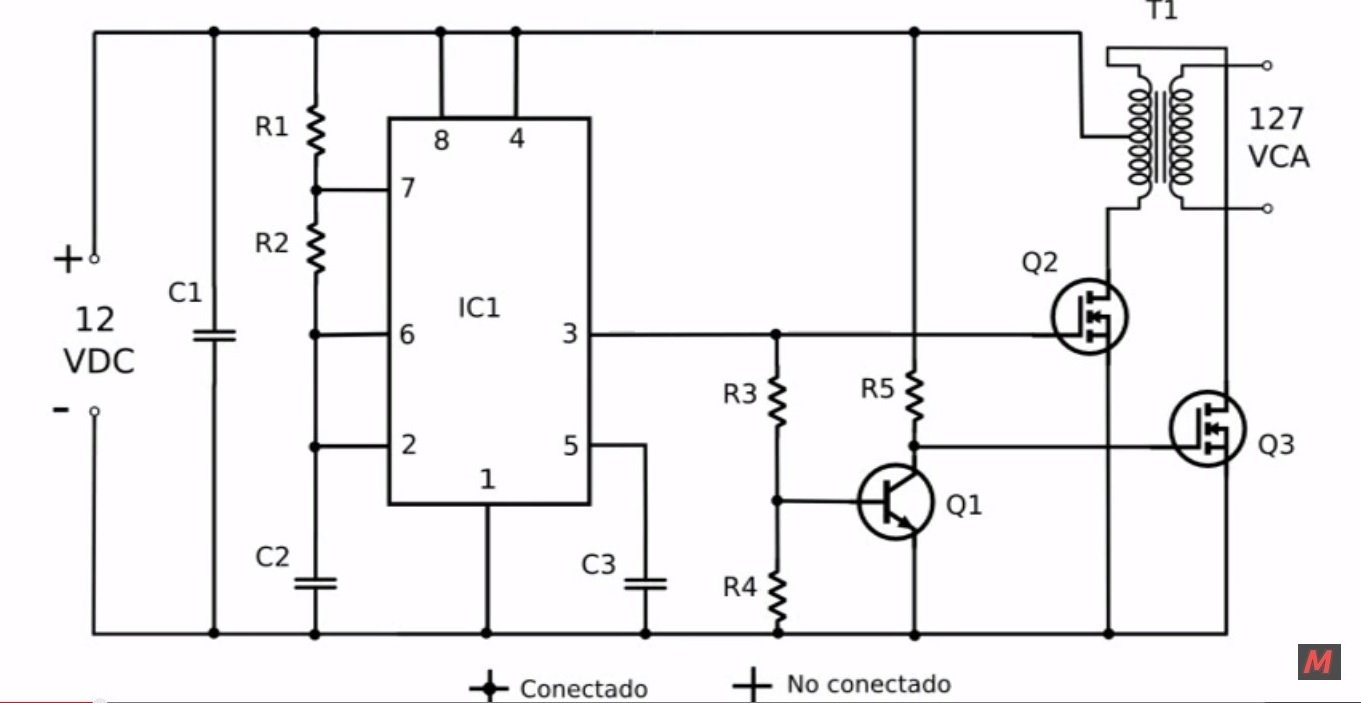
\includegraphics[scale=.30]{CD-CA.jpg}
\caption{}
\label{}
\end{figure}\\
Este circuito es de tres secciones: El oscilador, el distribuidor y la salida de potencia.
El oscilador est\'a conformado principlamente por el IC1, la frecuencia de oscilaci\'on est\'a determinada por R1, R2 y C2, el ajuste de esta est\'a a cargo de R1. En el pin 3 de IC1 est\'an presentes los pulsos que a trav\'es de R3 son entregados al pin 3 de IC2. El distribuidor, est\'a conformado por IC2, se encarga de alternar y amplificar los pulsos y entregarlos alternadamente a cada uno de los transistores Q1 y Q2.
La salida de potencia est\'a a cargo de Q1 Y Q2, quienes habiendo recibido los pulsos en sus bases a través de R5 y R6 respectivamente, los hacen pasar por el devanado primario de T1 e inducir una corriente y formar un campo magn\'etico que es transferido al secundario en el cual ya est\'a elevado.\\

\section{Convertidor de potencia CA-CA}
Este convertidor a partir de una tensi\'on de entrada alterna, produce en la salida una tensi\'on tambi\'en alterna pero de caracter\'isticas distintas, sea en valor eficaz, sea en frecuencia, o en ambas.Cuando \'unicamente se altera el valor de la tensi\'on alterna (CA), tenemos los llamados reguladores de tensi\'on alterna (o reguladores de potencia alterna) y los que permiten obtener una salida con frecuencia distinta a la presente en la entrada, son los cicloconvertidores.\\
\begin{figure}[htp]
\centering
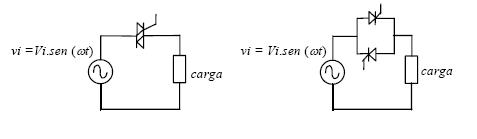
\includegraphics[scale=2.60]{circuito.jpg}
\caption{}
\label{}
\end{figure}
\begin{figure}[htp]
\centering
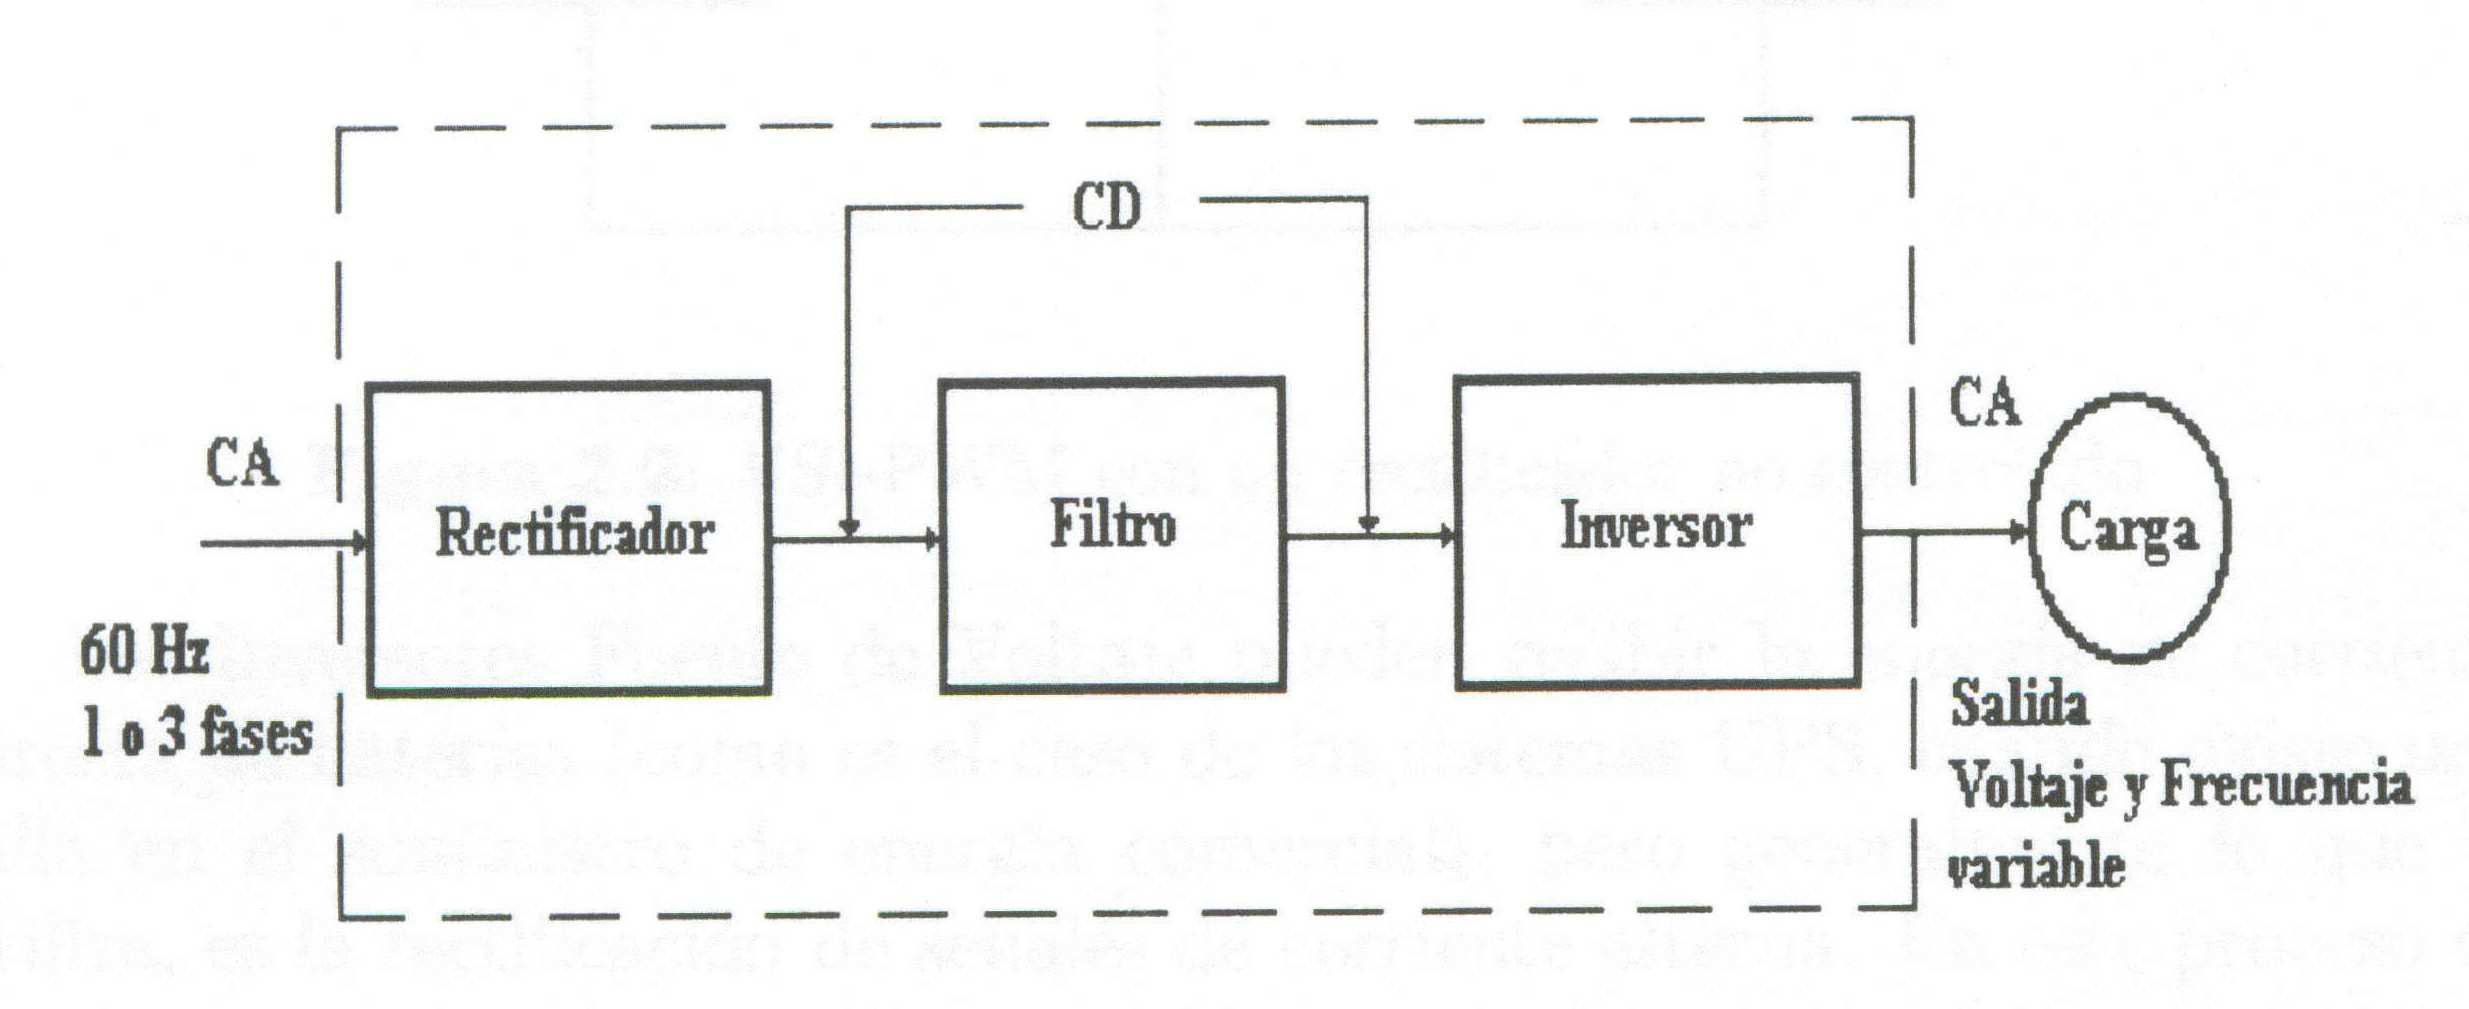
\includegraphics[scale=.10]{CA-CA.png}
\caption{}
\label{}
\end{figure}
\section{Convertidor de potencia CD-CD}
Los convertidores CD-CD o regulador de conmutaci\'on aporta dando a su salida una tensi\'on regulada y, la mayor\'ia de las veces con limitaci\'on de corriente. Se tiende a utilizar frecuencias de conmutaci\'on cada vez m\'as elevadas porque permiten reducir la capacidad de los condensadores, con el consiguiente beneficio de volumen, peso y precio.\\
\begin{figure}[htp]
\centering
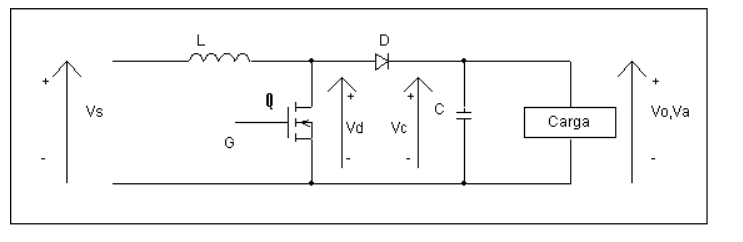
\includegraphics[scale=.50]{CD-CD.png}
\caption{}
\label{}
\end{figure}\\
Cuando  se  desconecta  el  transistor  Q  en  t  =  t1.  La  corriente  que  estaba  fluyendo  a  trav\'es  del  transistor  fluirá ahora a través de L, C, la carga y el Diodo D. La corriente del inductor se abate hasta que  se  vuelve  a  activar  en  el  siguiente  ciclo  del  transistor  Q.  La  energía  almacenada  en  el  inductor  L  es  transferida  a  la  carga  [1].
\begin{figure}[htp]
\centering
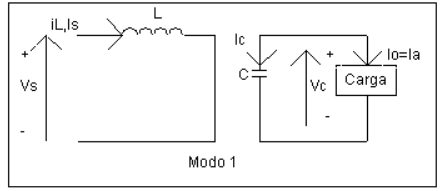
\includegraphics[scale=.70]{Cd-Cd.png}
\caption{}
\label{}
\end{figure}

\bibliography{Bibliografia .bib}{}
\bibliographystyle{plain}
\url {http://ccpot.galeon.com/enlaces1737112.html}\\
\url {https://es.scribd.com/document/283902697/convertidores-CD-CA}\\
\url {https://www.researchgate.net/figure/Circuito-de-control-principal-El-nucleo-del-sistema-es-un-microcontrolador-PIC16F873_fig6_313423325}\\
\url  { http://catarina.udlap.mx/u_dl_a/tales/documentos/lem/martinez_v_da/capitulo2.pdf}\\
\url {https://prezi.com/k71cj-csevjr/convertidores-cd-cd/}\\
\end{document}
